\chapter{System Walkthrough: Web UI and Experiment Tracking}
\label{app:walkthrough}

This appendix illustrates the running system referenced from Chapter~\ref{chap:implementation}. It walks through the serving path (the FastAPI dashboard) on two contrasting sessions and then through the two MLflow experiments that track the serving and batch paths. The two sessions show both ends of the label-optional design: a labeled session, where the dashboard additionally computes evaluation metrics, and an unlabeled session, where only the proxy monitoring signals are available. The screenshots confirm that the behavior described in Chapters~\ref{chap:implementation}--\ref{chap:experiments} operates in the live system; they are presented as evidence of the implementation, not as a separate argument.

\section{Serving Path on a Labeled Session}
\label{app:walkthrough_labeled}

Figure~\ref{fig:appF_labeled} walks through the serving path on the labeled User~7 session (fused upload mode), from upload to per-window predictions. Because the upload carries ground-truth labels, the dashboard computes an evaluation card (accuracy, macro-F1, and their smoothed variants) in addition to the monitoring signals, and the temporal signal routes the run to review. Key things to observe: the stage strip at the top of the upload screen (S1--S3 preprocessing, S4--S7 result path, S8--S10 review-gated) mirrors the ten-stage architecture of Chapter~\ref{chap:implementation}; the evaluation card appears only in this labeled mode and is absent in the unlabeled case below; and the governance decision is \texttt{REVIEW} because the raw temporal transition rate (40.6\%) exceeds the monitoring threshold even though the smoothed rate (21.5\%) is below it, which is the expected separation between the monitoring and serving paths described in Section~\ref{sec:ch7_sessions25}.

\begin{figure}[htbp]
\centering
\begin{subfigure}{\textwidth}\centering
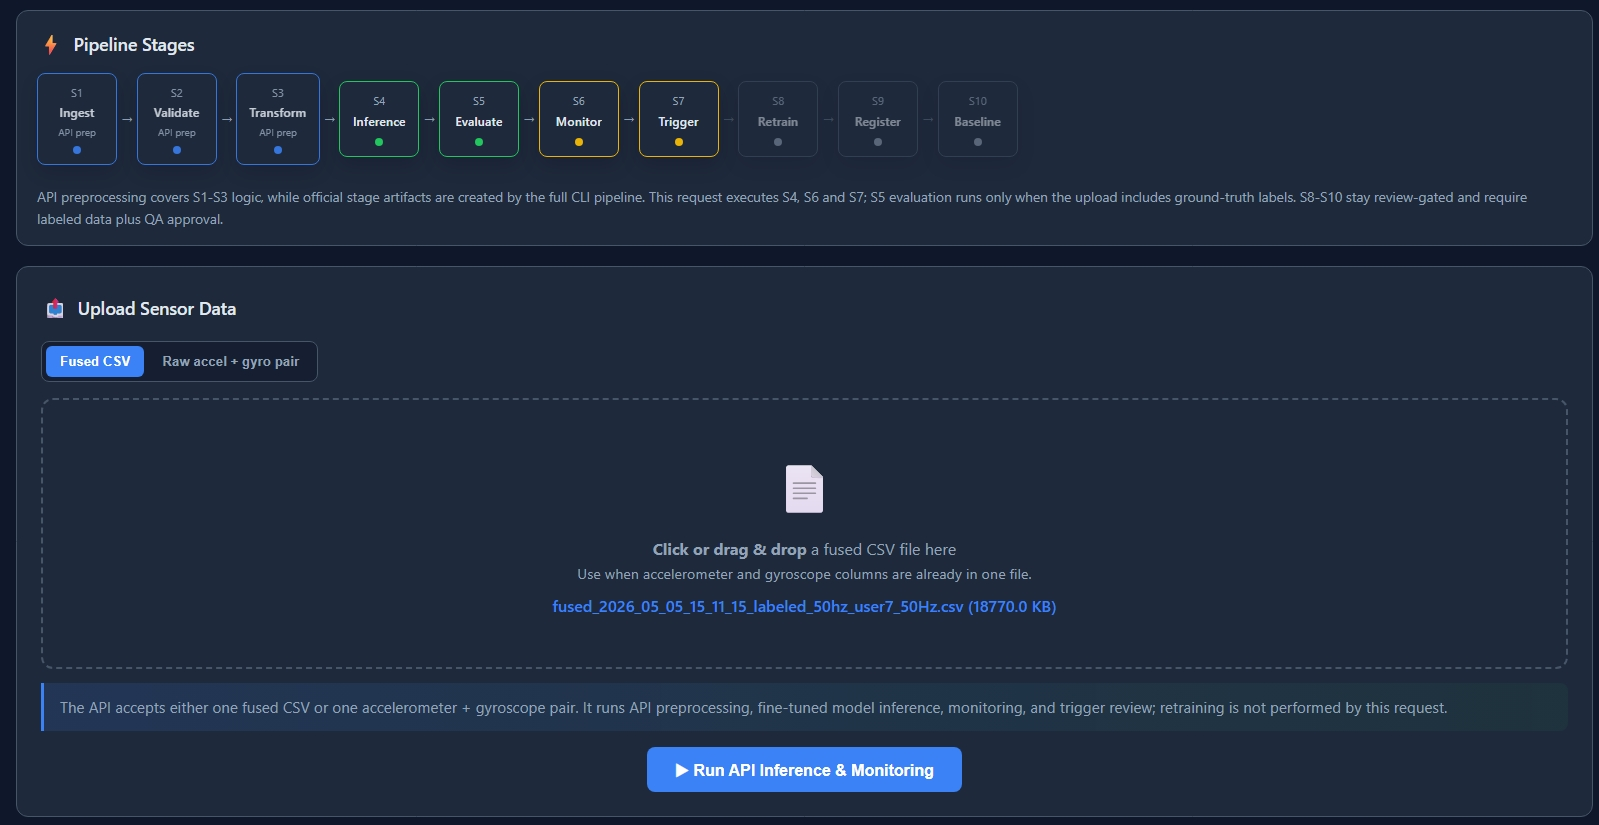
\includegraphics[width=0.79\textwidth]{figures/fig_appF_labeled_upload.jpeg}
\caption{Upload screen with the stage strip (S1--S3 API preprocessing, S4--S7 visible result path, S8--S10 review-gated) and the fused-CSV upload mode.}
\label{fig:appF_labeled_upload}
\end{subfigure}\\[1.0ex]
\begin{subfigure}{\textwidth}\centering
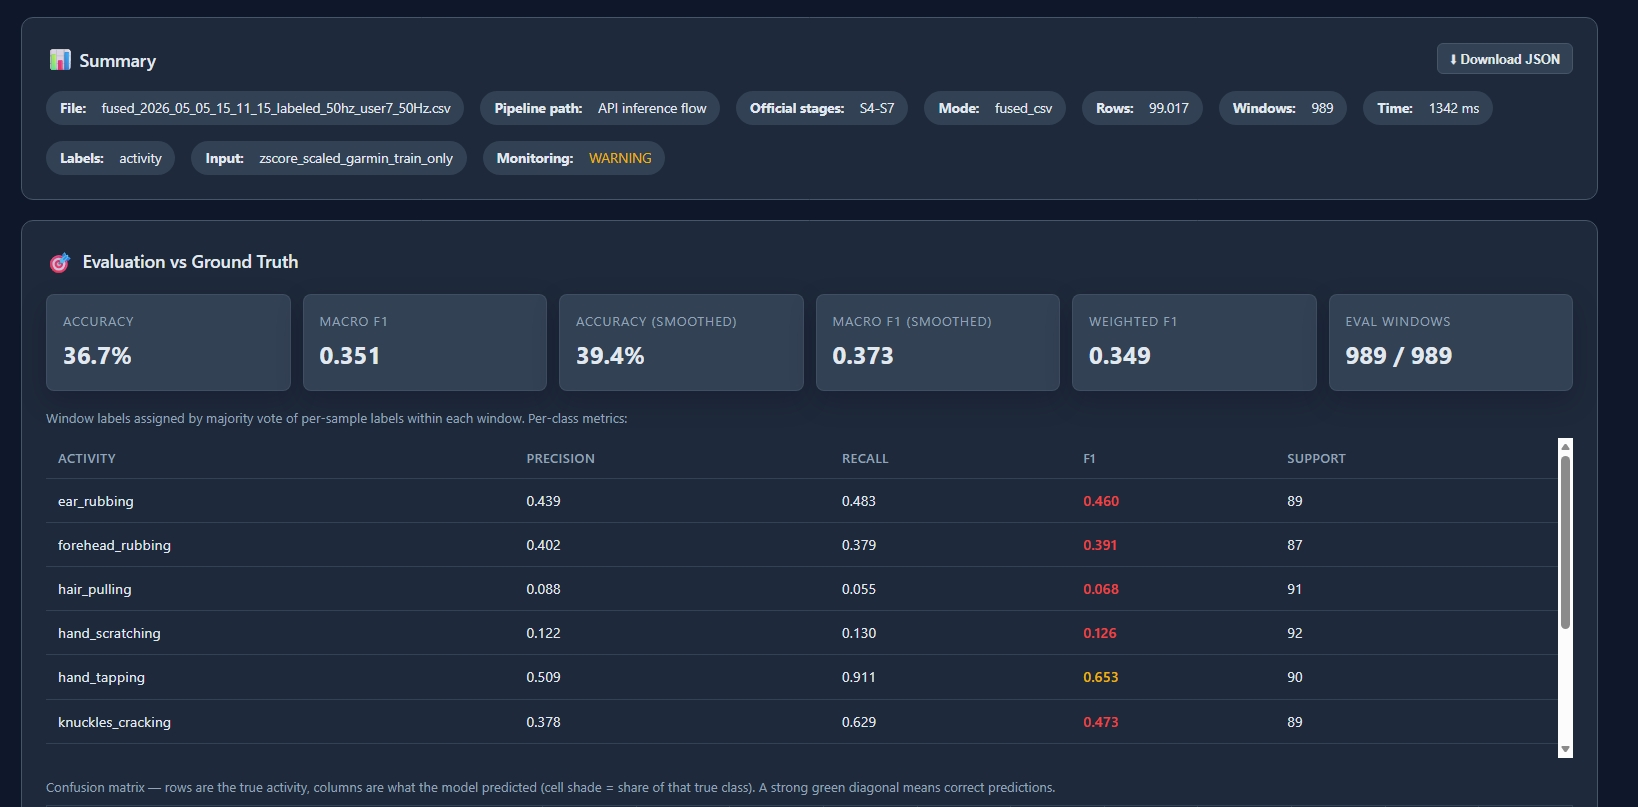
\includegraphics[width=0.79\textwidth]{figures/fig_appF_labeled_summary.jpeg}
\caption{Run summary (API inference flow, stages S4--S7, fused mode, 989 windows) and the labeled evaluation card with accuracy, macro-F1, and smoothed variants.}
\label{fig:appF_labeled_summary}
\end{subfigure}\\[1.0ex]
\begin{subfigure}{\textwidth}\centering
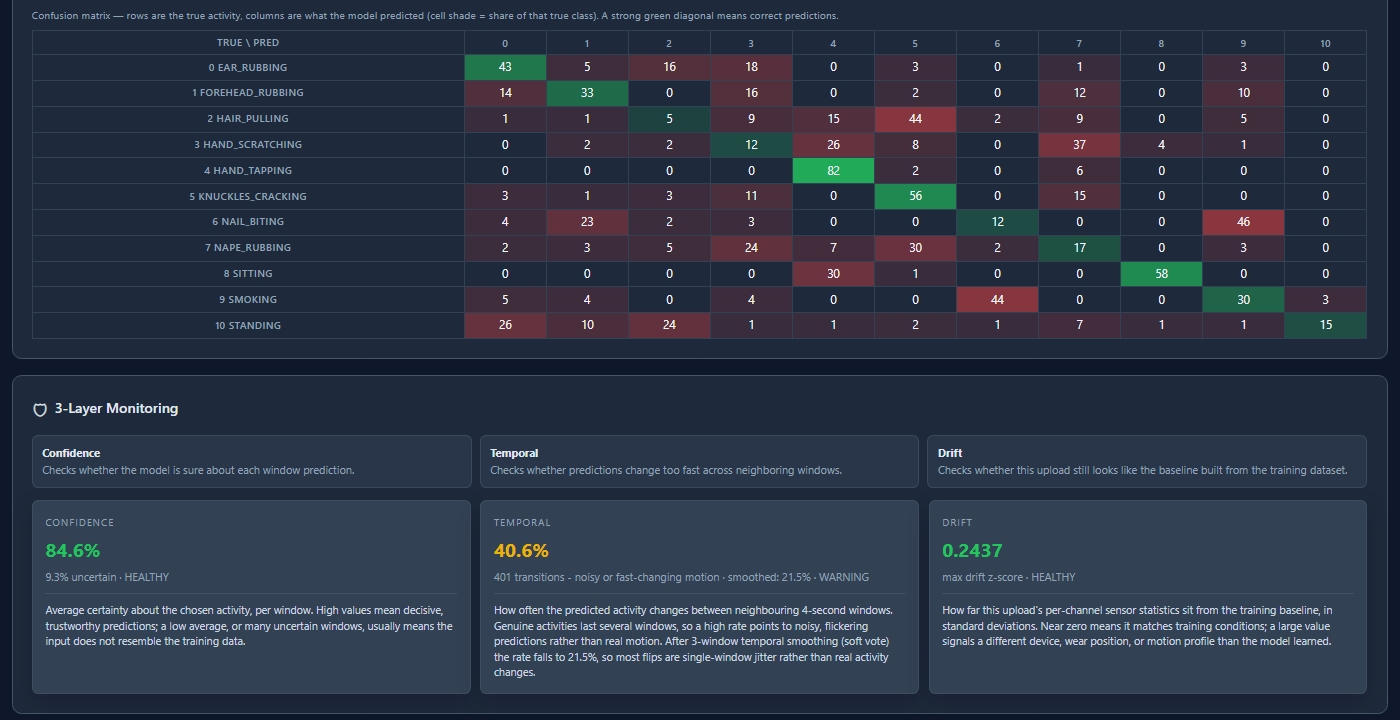
\includegraphics[width=0.79\textwidth]{figures/fig_appF_labeled_monitoring.jpeg}
\caption{Three-layer monitoring (confidence 84.6\%, temporal 40.6\% with smoothed 21.5\%, drift $z=0.24$) and the per-class confusion matrix.}
\label{fig:appF_labeled_monitoring}
\end{subfigure}
\caption[Serving path on a labeled session (User~7), part~1]{Serving path on the labeled User~7 session (continued in Figure~\ref{fig:appF_labeled2}). The evaluation card is computed only because the upload carried labels.}
\label{fig:appF_labeled}
\end{figure}

\begin{figure}[htbp]\ContinuedFloat
\centering
\begin{subfigure}{\textwidth}\centering
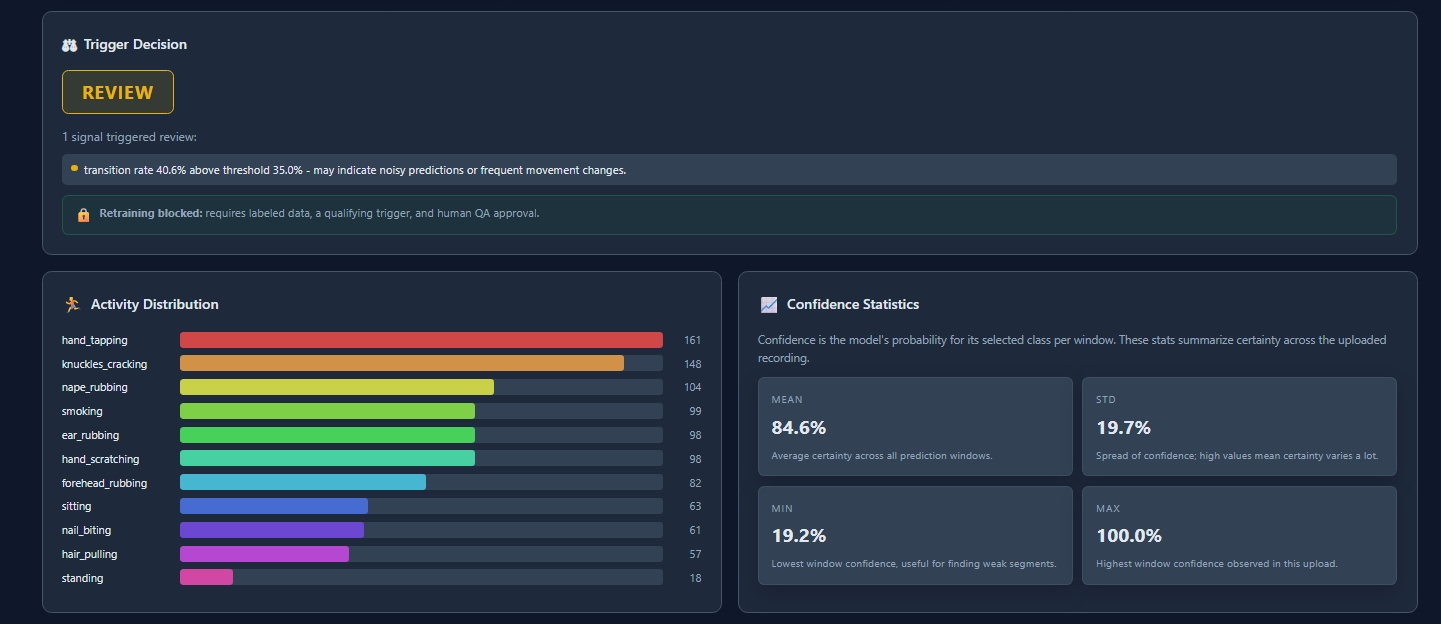
\includegraphics[width=0.94\textwidth]{figures/fig_appF_labeled_trigger.jpeg}
\caption{Governance decision: routed to \texttt{REVIEW} by the temporal signal, with retraining blocked pending labels, a qualifying trigger, and human approval.}
\label{fig:appF_labeled_trigger}
\end{subfigure}\\[1.0ex]
\begin{subfigure}{\textwidth}\centering
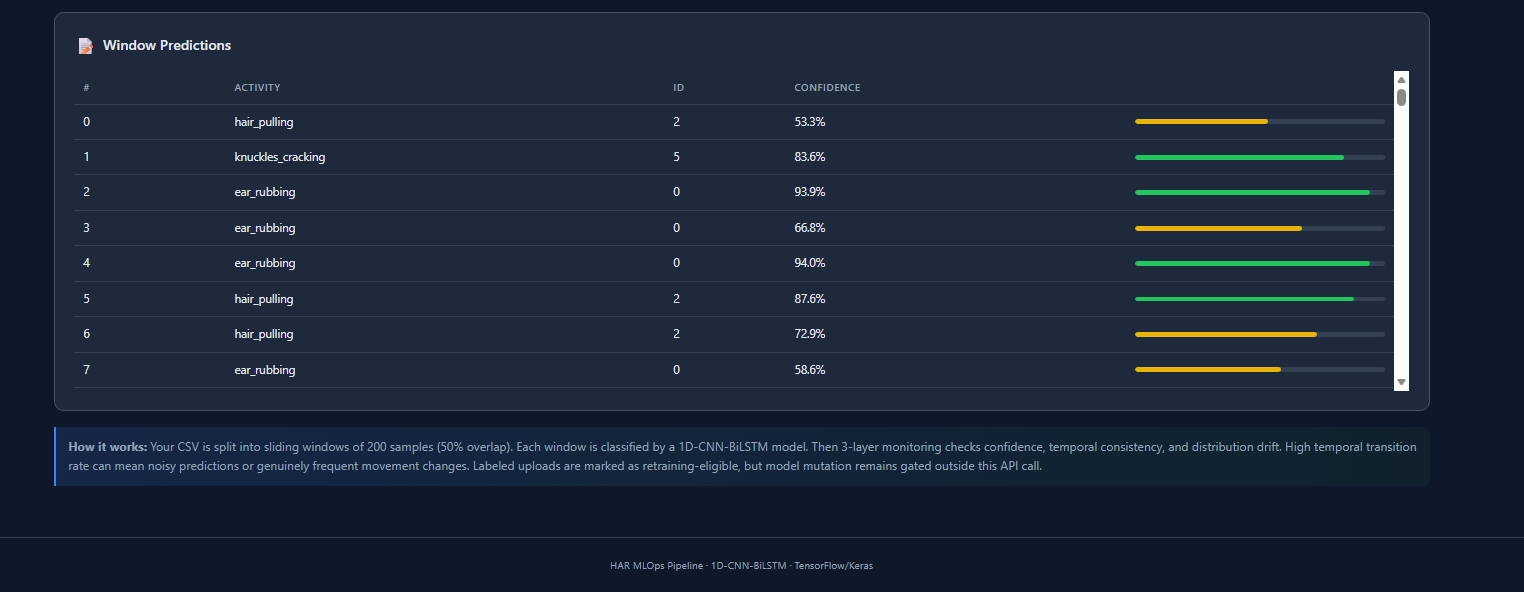
\includegraphics[width=0.94\textwidth]{figures/fig_appF_labeled_predictions.jpeg}
\caption{Per-window predictions with confidence, and the footer explaining the windowing and three-layer monitoring contract.}
\label{fig:appF_labeled_predictions}
\end{subfigure}
\caption[Serving path on a labeled session (User~7), part~2]{Serving path on the labeled User~7 session (continued). The temporal signal routes the run to review while retraining stays blocked, the no-auto-retrain invariant of Chapter~\ref{chap:monitoring} operating on live data.}
\label{fig:appF_labeled2}
\end{figure}
\FloatBarrier

\section{Serving Path on an Unlabeled Session}
\label{app:walkthrough_unlabeled}

Figure~\ref{fig:appF_unlabeled} shows the same serving path on an unlabeled session uploaded as a raw accelerometer-plus-gyroscope pair. No evaluation card is produced, because no ground truth exists; the pipeline relies entirely on the proxy monitoring signals. Here all three layers are healthy and the governance decision is \texttt{NO\_ACTION}, the complementary outcome to the labeled session above and the label-free monitoring behavior on which Section~\ref{sec:ch7_sessions25} reports at scale. Comparing these two sessions side by side illustrates the label-optional design: the upload interface, preprocessing, inference, monitoring, and governance stages all execute identically; the only difference is that the labeled session additionally activates the evaluation card, and its elevated temporal rate triggers a review while the unlabeled session's lower rate does not.

\begin{figure}[htbp]
\centering
\begin{subfigure}{\textwidth}\centering
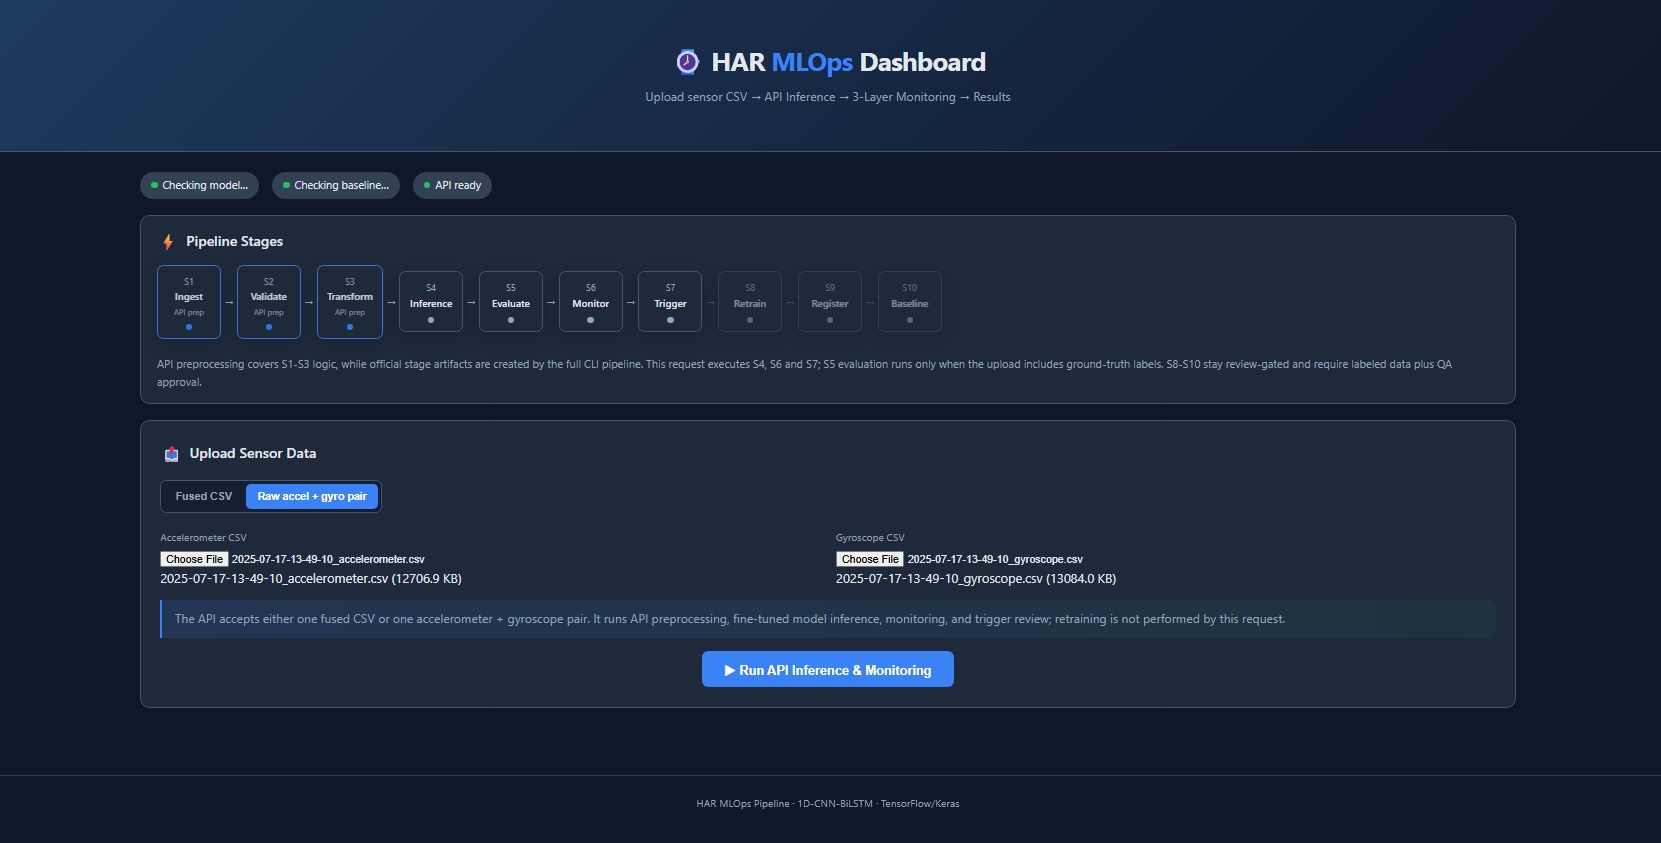
\includegraphics[width=0.94\textwidth]{figures/fig_appF_unlabeled_upload.jpeg}
\caption{Upload screen in raw accelerometer-plus-gyroscope mode, with the two-file picker.}
\label{fig:appF_unlabeled_upload}
\end{subfigure}\\[1.0ex]
\begin{subfigure}{\textwidth}\centering
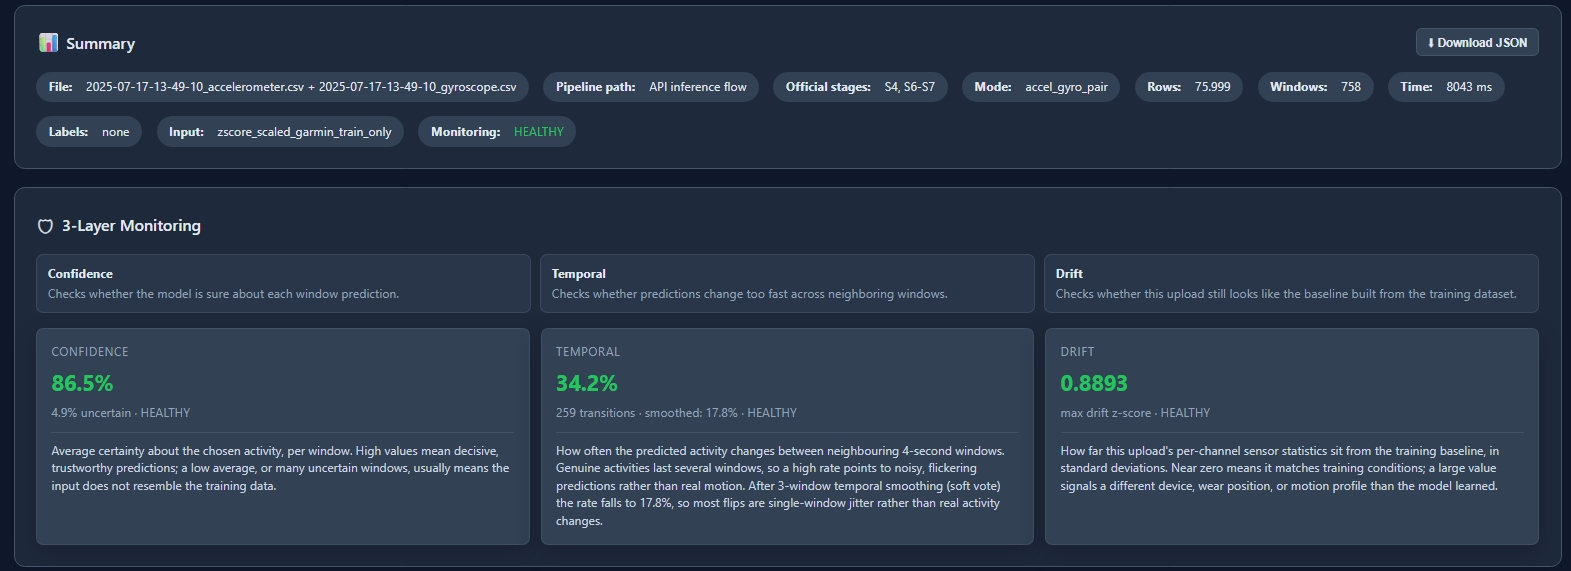
\includegraphics[width=0.94\textwidth]{figures/fig_appF_unlabeled_monitoring.jpeg}
\caption{Run summary (\texttt{Labels: none}, raw accel+gyro mode, 758 windows) and three-layer monitoring: confidence 86.5\%, temporal 34.2\% (smoothed 17.8\%), drift $z=0.89$, all healthy.}
\label{fig:appF_unlabeled_monitoring}
\end{subfigure}
\caption[Serving path on an unlabeled session, part~1]{Serving path on an unlabeled session (continued in Figure~\ref{fig:appF_unlabeled2}). With no labels, the dashboard produces no evaluation card and depends only on the proxy monitoring signals.}
\label{fig:appF_unlabeled}
\end{figure}

\begin{figure}[htbp]\ContinuedFloat
\centering
\begin{subfigure}{\textwidth}\centering
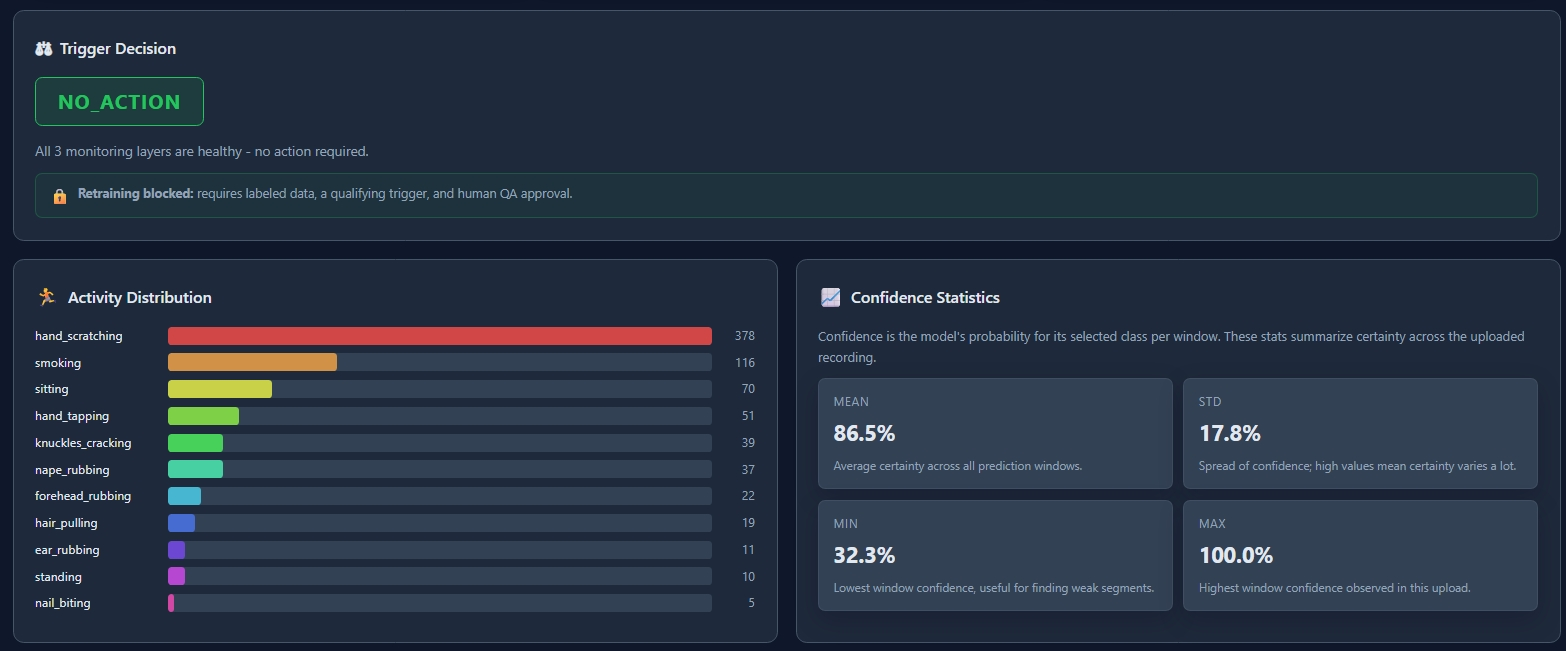
\includegraphics[width=0.94\textwidth]{figures/fig_appF_unlabeled_trigger.jpeg}
\caption{Governance decision: \texttt{NO\_ACTION}, since all three monitoring layers are healthy; retraining remains blocked by the same gate.}
\label{fig:appF_unlabeled_trigger}
\end{subfigure}\\[1.0ex]
\begin{subfigure}{\textwidth}\centering
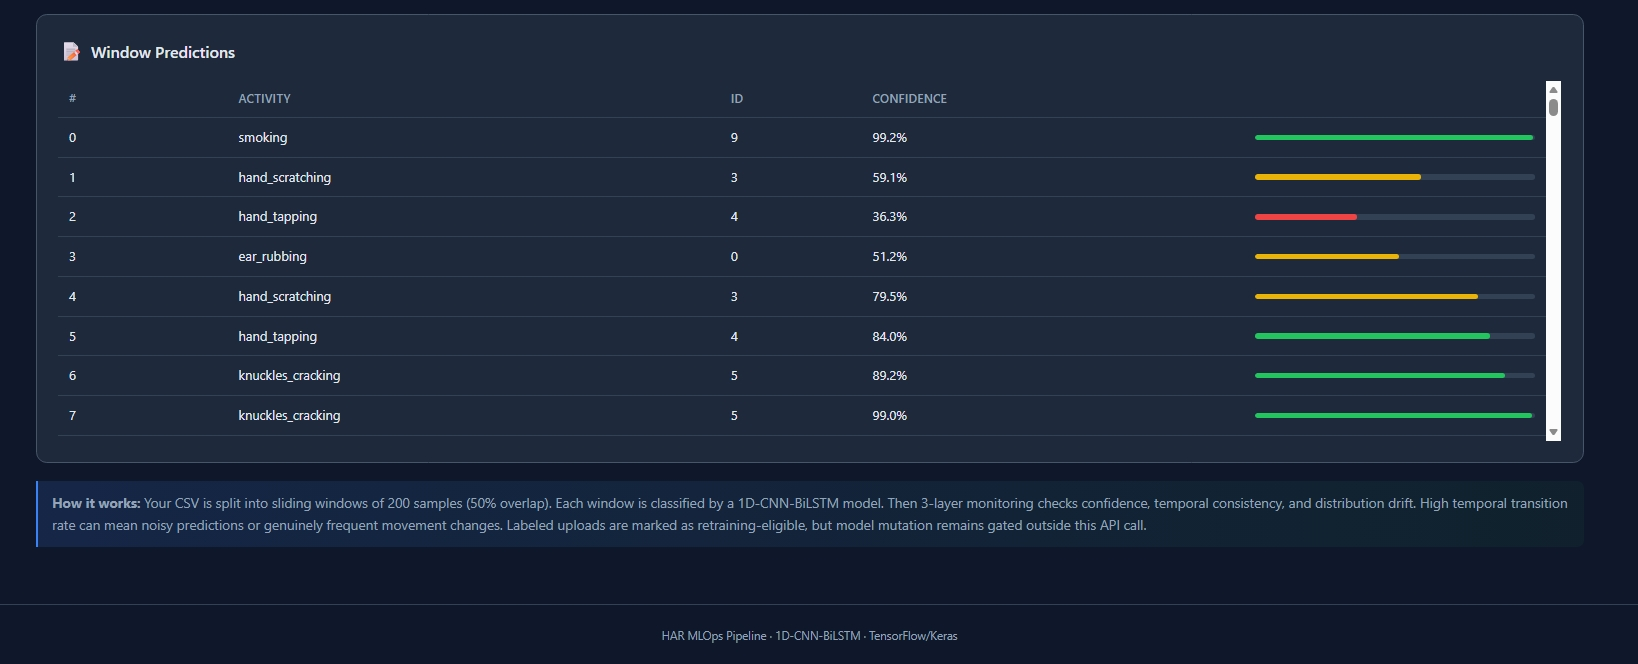
\includegraphics[width=0.94\textwidth]{figures/fig_appF_unlabeled_predictions.jpeg}
\caption{Per-window predictions with confidence for the unlabeled session.}
\label{fig:appF_unlabeled_predictions}
\end{subfigure}
\caption[Serving path on an unlabeled session, part~2]{Serving path on an unlabeled session (continued). All layers are healthy and the trigger returns \texttt{NO\_ACTION}, the complement to the labeled review case in Figure~\ref{fig:appF_labeled2}.}
\label{fig:appF_unlabeled2}
\end{figure}
\FloatBarrier

\section{Experiment Tracking}
\label{app:walkthrough_mlflow}

MLflow records the two execution paths of Section~\ref{sec:experiment_tracking} as two separate experiments, shown in Figure~\ref{fig:appF_experiments}. The remainder of this section tours each experiment in turn, from its run list through a single run's overview, curated metrics and parameters, and logged artifacts. Keeping the serving and batch paths in separate experiments prevents interactive dashboard submissions from diluting the governed batch-run history; each experiment therefore provides a clean, queryable record of its own execution path and makes the audit trail described in Section~\ref{sec:run_scoped_artifacts} navigable without filtering.

\begin{figure}[htbp]
\centering
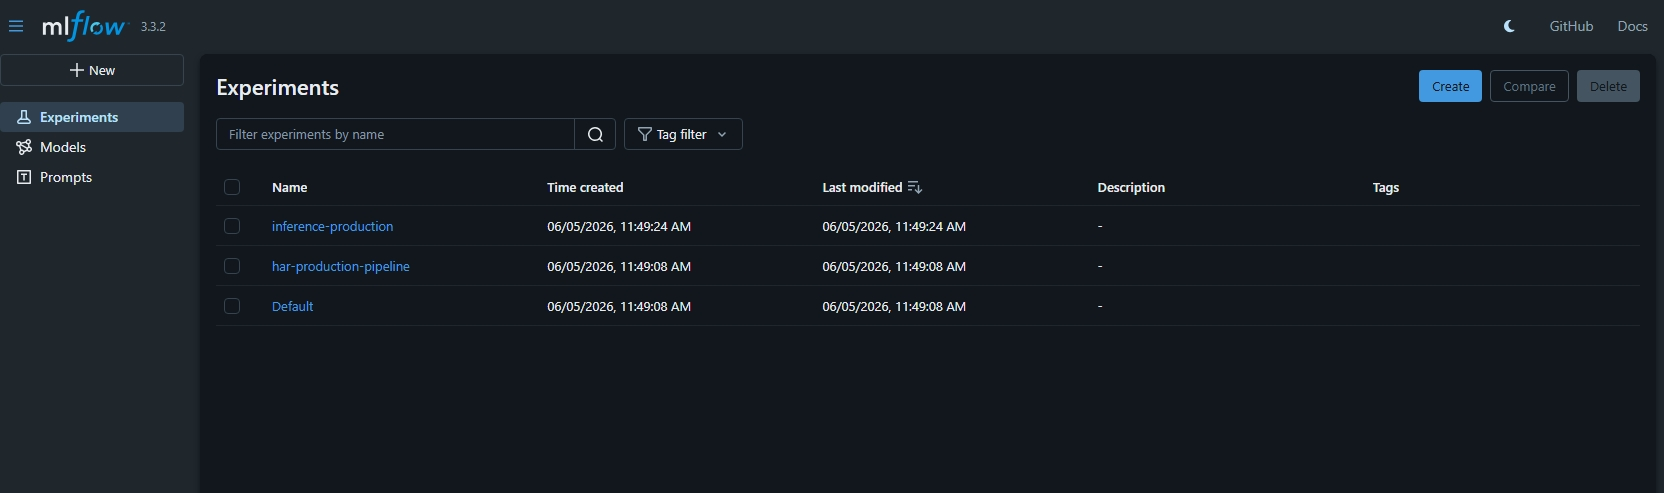
\includegraphics[width=0.94\textwidth]{figures/fig_appF_pipe_experiments.jpeg}
\caption[MLflow experiments for the two execution paths]{The two execution paths recorded as separate MLflow experiments: \texttt{inference-production} (serving) and \texttt{har-production-pipeline} (batch). Keeping them separate prevents interactive serving runs from diluting the governed batch-run history.}
\label{fig:appF_experiments}
\end{figure}
\FloatBarrier

\subsection{Inference-Production Experiment (Serving Path)}
\label{app:walkthrough_inf}

The \texttt{inference-production} experiment captures runs from two sources: the Stage~4 batch inference logger (\path{src/components/model_inference.py}), which records the resolved contract (model MD5, scaler input space, runtime mode) and archives the inference report and prediction files; and the WebUI logger (\path{_log_inference_mlflow()} in \path{src/api/app.py}), which records the proxy monitoring metrics (mean confidence, per-activity counts, total windows) for dashboard-submitted sessions. Figure~\ref{fig:appF_inf} tours a single batch-path run, where both metric and parameter sets are present.

\begin{figure}[htbp]
\centering
\begin{subfigure}{\textwidth}\centering
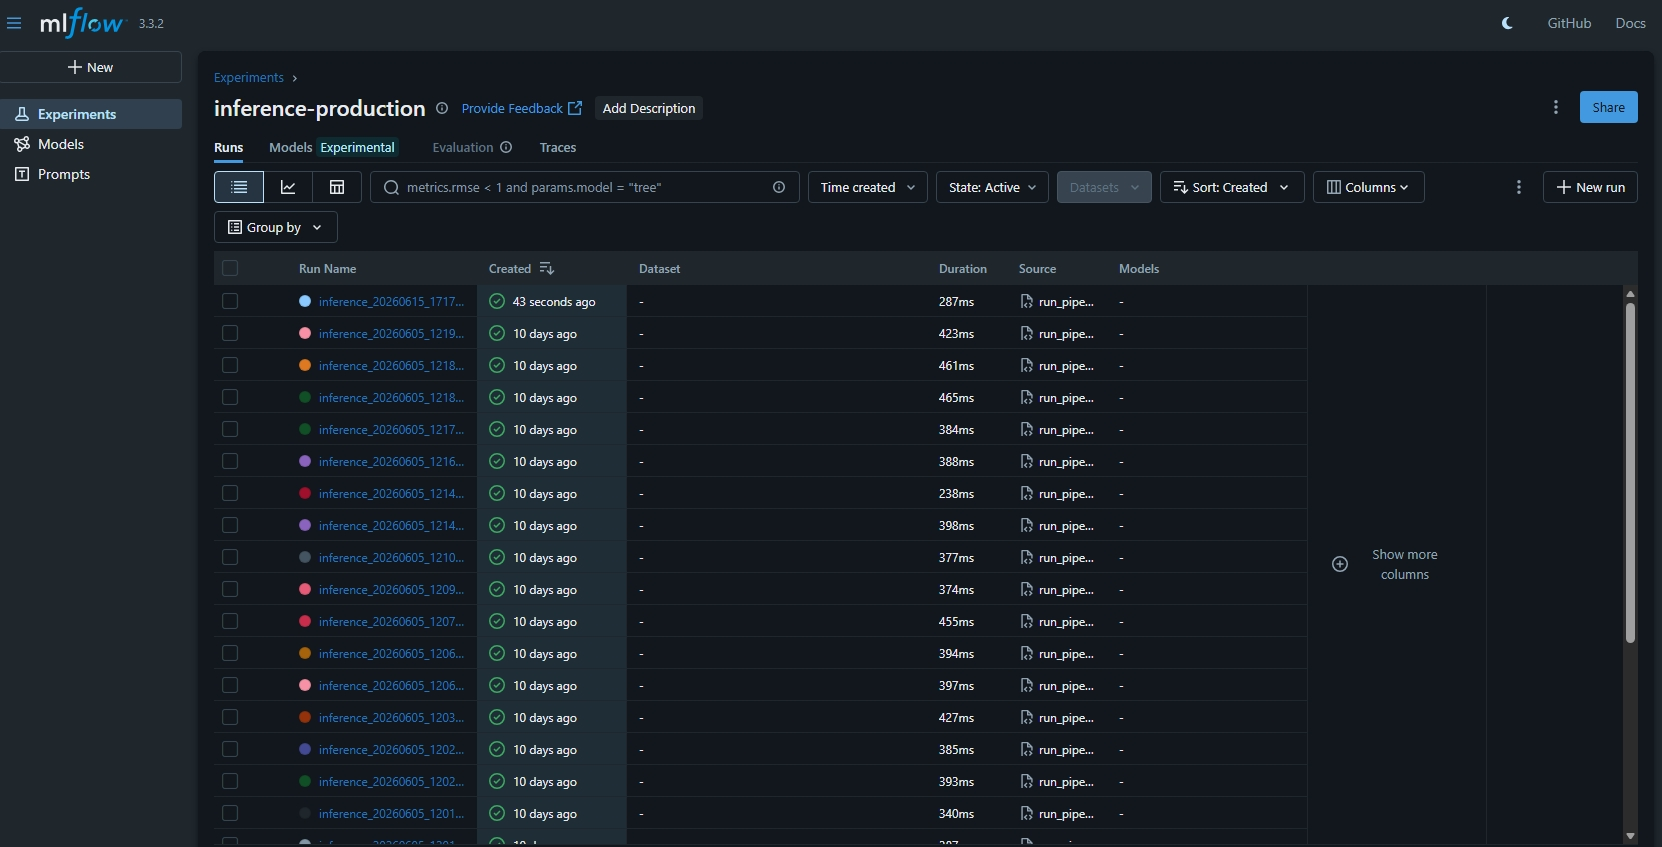
\includegraphics[width=0.94\textwidth]{figures/fig_appF_inf_runs.jpeg}
\caption{Run list of the \texttt{inference-production} experiment (serving-path uploads).}
\label{fig:appF_inf_runs}
\end{subfigure}\\[1.0ex]
\begin{subfigure}{\textwidth}\centering
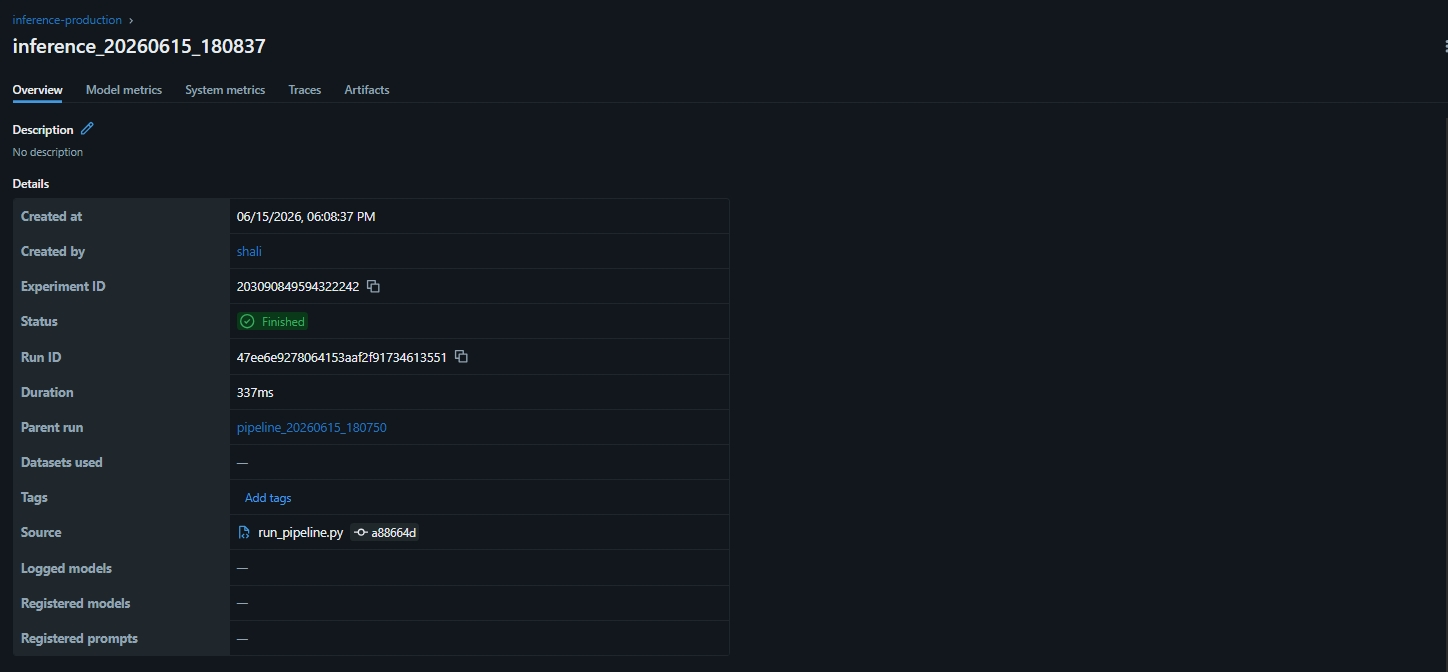
\includegraphics[width=0.94\textwidth]{figures/fig_appF_inf_overview.jpeg}
\caption{Run overview: run identifier, finished status, source script and commit, and the parent-run link tying serving evidence back to its pipeline run.}
\label{fig:appF_inf_overview}
\end{subfigure}
\caption[Inference-production experiment, part~1]{Inference-production experiment (continued in Figure~\ref{fig:appF_inf2}): run list and single-run provenance.}
\label{fig:appF_inf}
\end{figure}

\begin{figure}[htbp]\ContinuedFloat
\centering
\begin{subfigure}{\textwidth}\centering
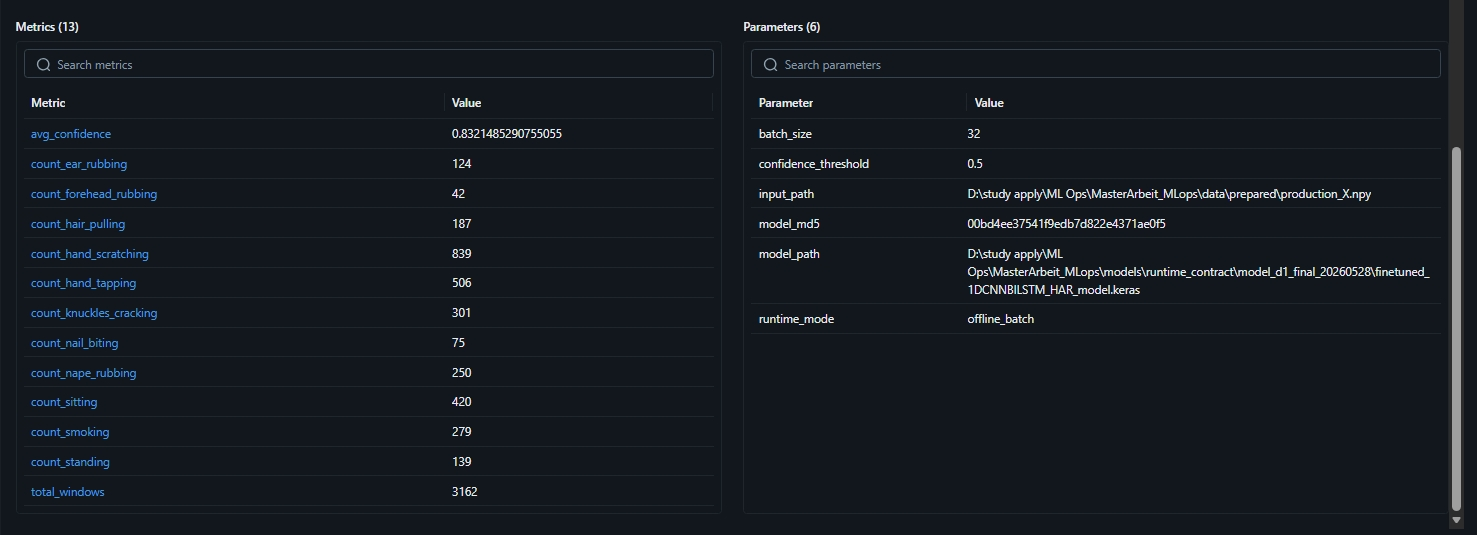
\includegraphics[width=0.94\textwidth]{figures/fig_appF_inf_metrics.jpeg}
\caption{Metrics tab: mean confidence, per-activity counts, and total windows (proxy set). Parameters tab: model MD5, scaler input space, and runtime mode (Stage~4 batch logger).}
\label{fig:appF_inf_metrics}
\end{subfigure}\\[1.0ex]
\begin{subfigure}{\textwidth}\centering
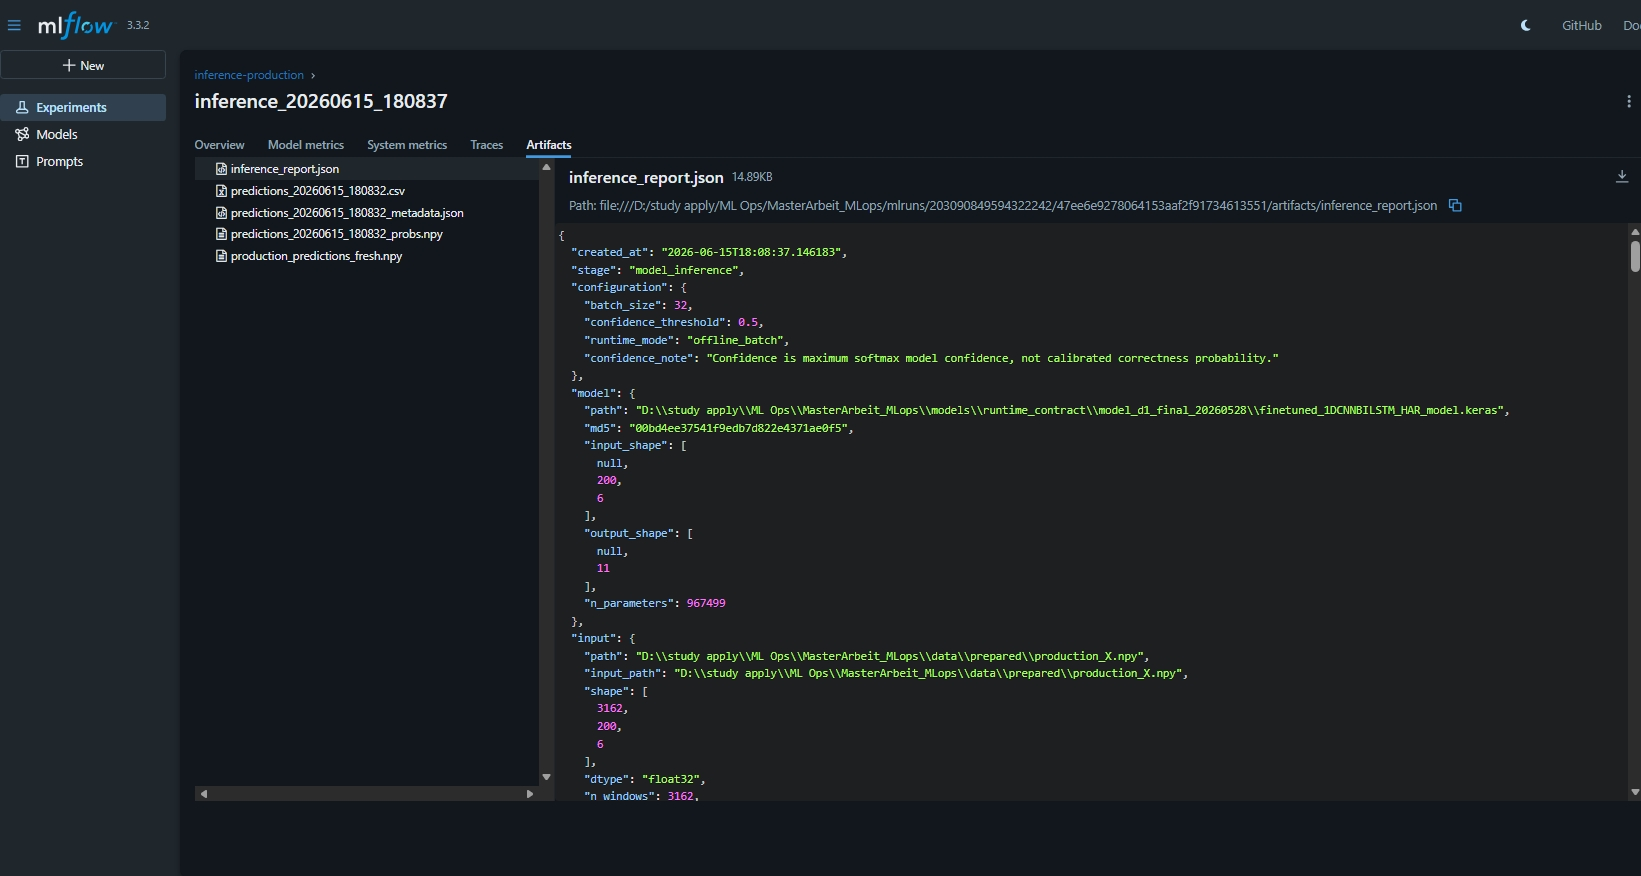
\includegraphics[width=0.94\textwidth]{figures/fig_appF_inf_artifacts.jpeg}
\caption{Logged artifacts: the inference report and prediction files archived with the run.}
\label{fig:appF_inf_artifacts}
\end{subfigure}
\caption[Inference-production experiment, part~2]{Inference-production experiment (continued): curated metrics and parameters, and the archived artifacts.}
\label{fig:appF_inf2}
\end{figure}
\FloatBarrier

\subsection{Har-Production-Pipeline Experiment (Batch Path)}
\label{app:walkthrough_pipe}

Figure~\ref{fig:appF_pipe} tours a single batch run. The metrics tab (\ref{fig:appF_pipe_metrics}) shows the curated thirteen stage metrics of Section~\ref{sec:experiment_tracking}, one or two per stage, together with run parameters recording that all seven stages completed, the overall status was \texttt{SUCCESS}, and every retraining flag was \texttt{False}, the no-auto-retrain outcome captured as data. The artifacts tab exposes \texttt{run\_info.json}, which records each stage's status and details and is the run-scoped artifact trail of Section~\ref{sec:run_scoped_artifacts}.

\begin{figure}[htbp]
\centering
\begin{subfigure}{\textwidth}\centering
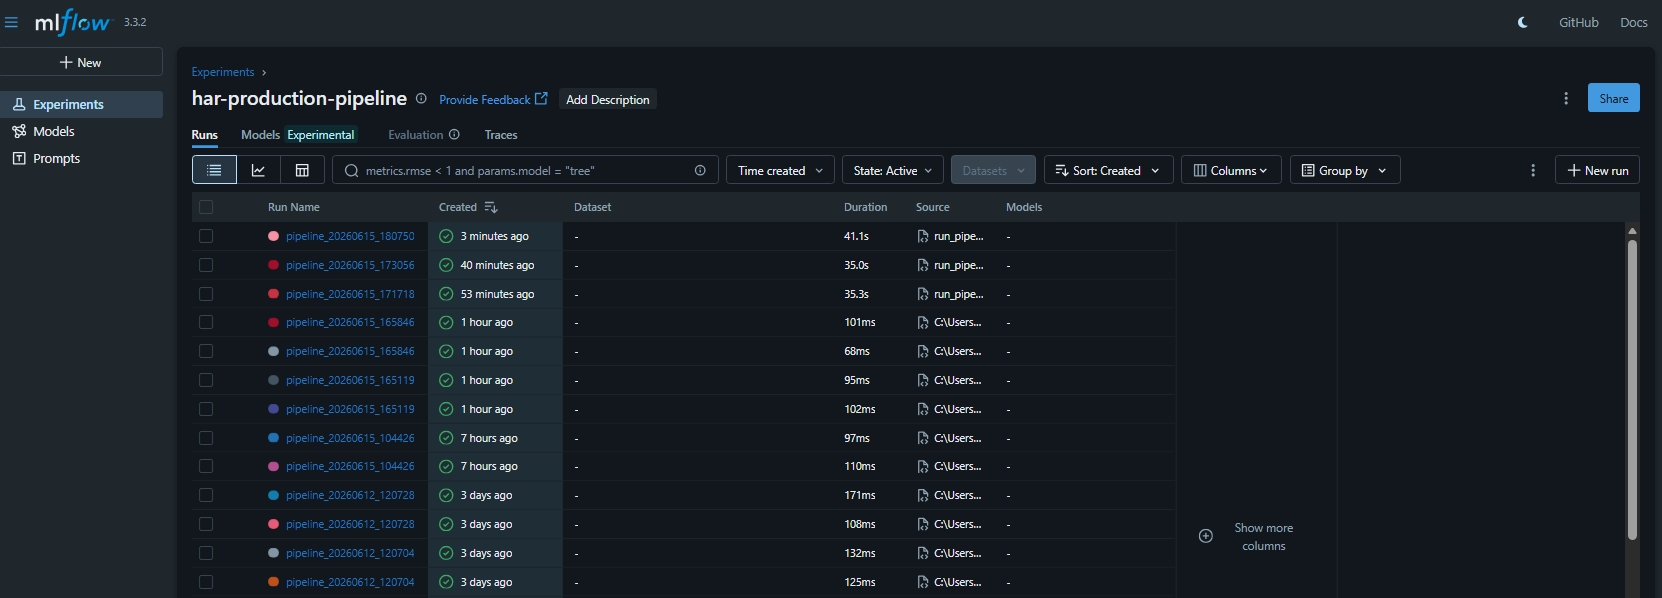
\includegraphics[width=0.94\textwidth]{figures/fig_appF_pipe_runs.jpeg}
\caption{Run list of the \texttt{har-production-pipeline} experiment (governed batch runs).}
\label{fig:appF_pipe_runs}
\end{subfigure}\\[1.0ex]
\begin{subfigure}{\textwidth}\centering
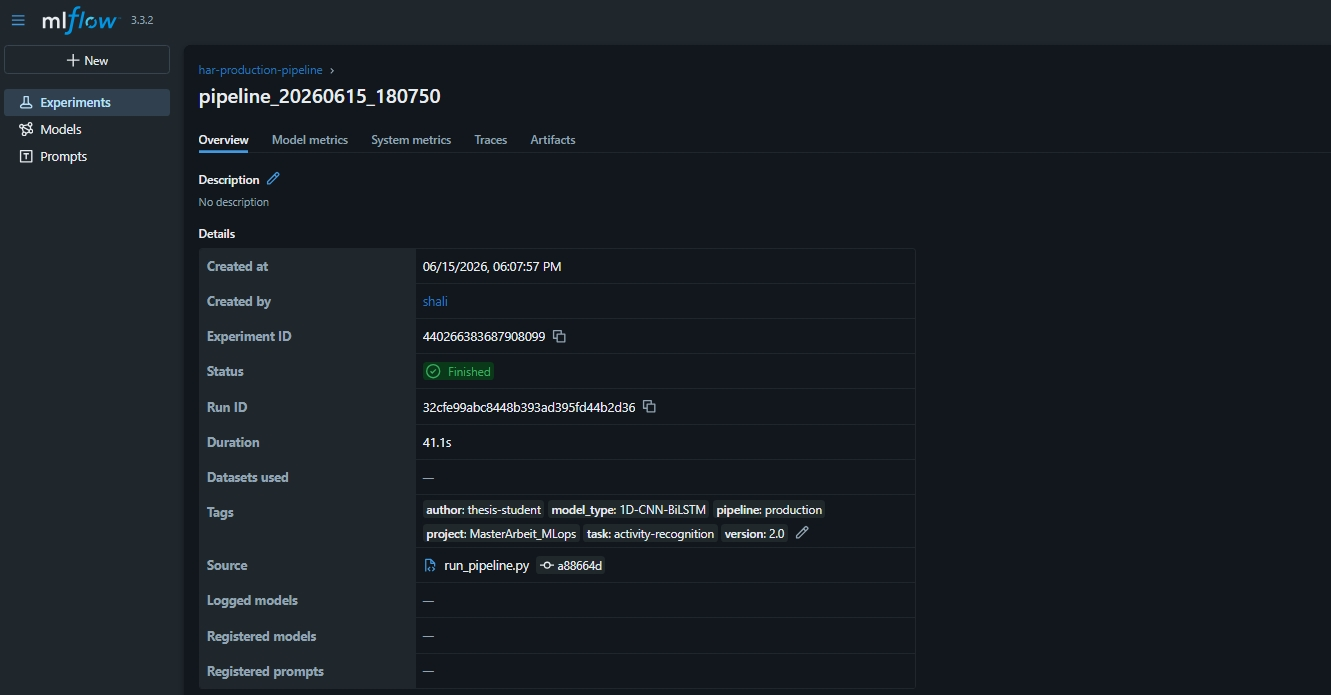
\includegraphics[width=0.94\textwidth]{figures/fig_appF_pipe_overview.jpeg}
\caption{Run overview with run-level tags (author, model type, task, version) and the source commit.}
\label{fig:appF_pipe_overview}
\end{subfigure}
\caption[Har-production-pipeline experiment, part~1]{Har-production-pipeline experiment (continued in Figure~\ref{fig:appF_pipe2}): run list and tagged provenance.}
\label{fig:appF_pipe}
\end{figure}

\begin{figure}[htbp]\ContinuedFloat
\centering
\begin{subfigure}{\textwidth}\centering
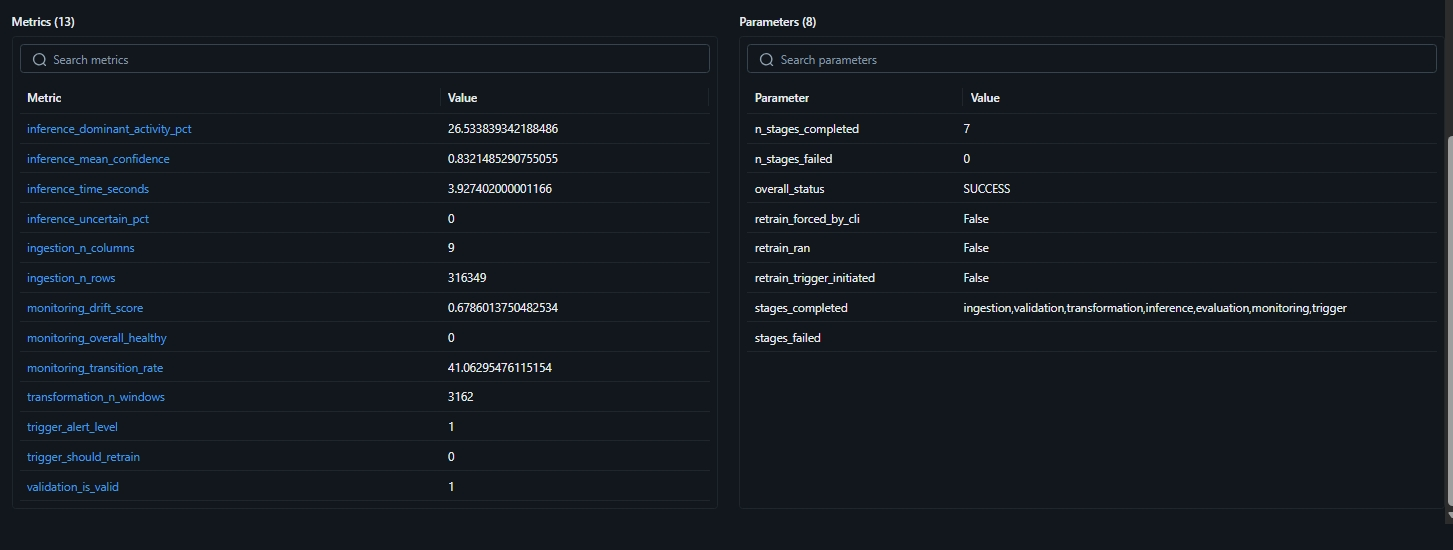
\includegraphics[width=0.94\textwidth]{figures/fig_appF_pipe_metrics.jpeg}
\caption{The thirteen curated stage metrics and run parameters: seven stages completed, \texttt{overall\_status=SUCCESS}, all retrain flags \texttt{False}.}
\label{fig:appF_pipe_metrics}
\end{subfigure}\\[1.0ex]
\begin{subfigure}{\textwidth}\centering
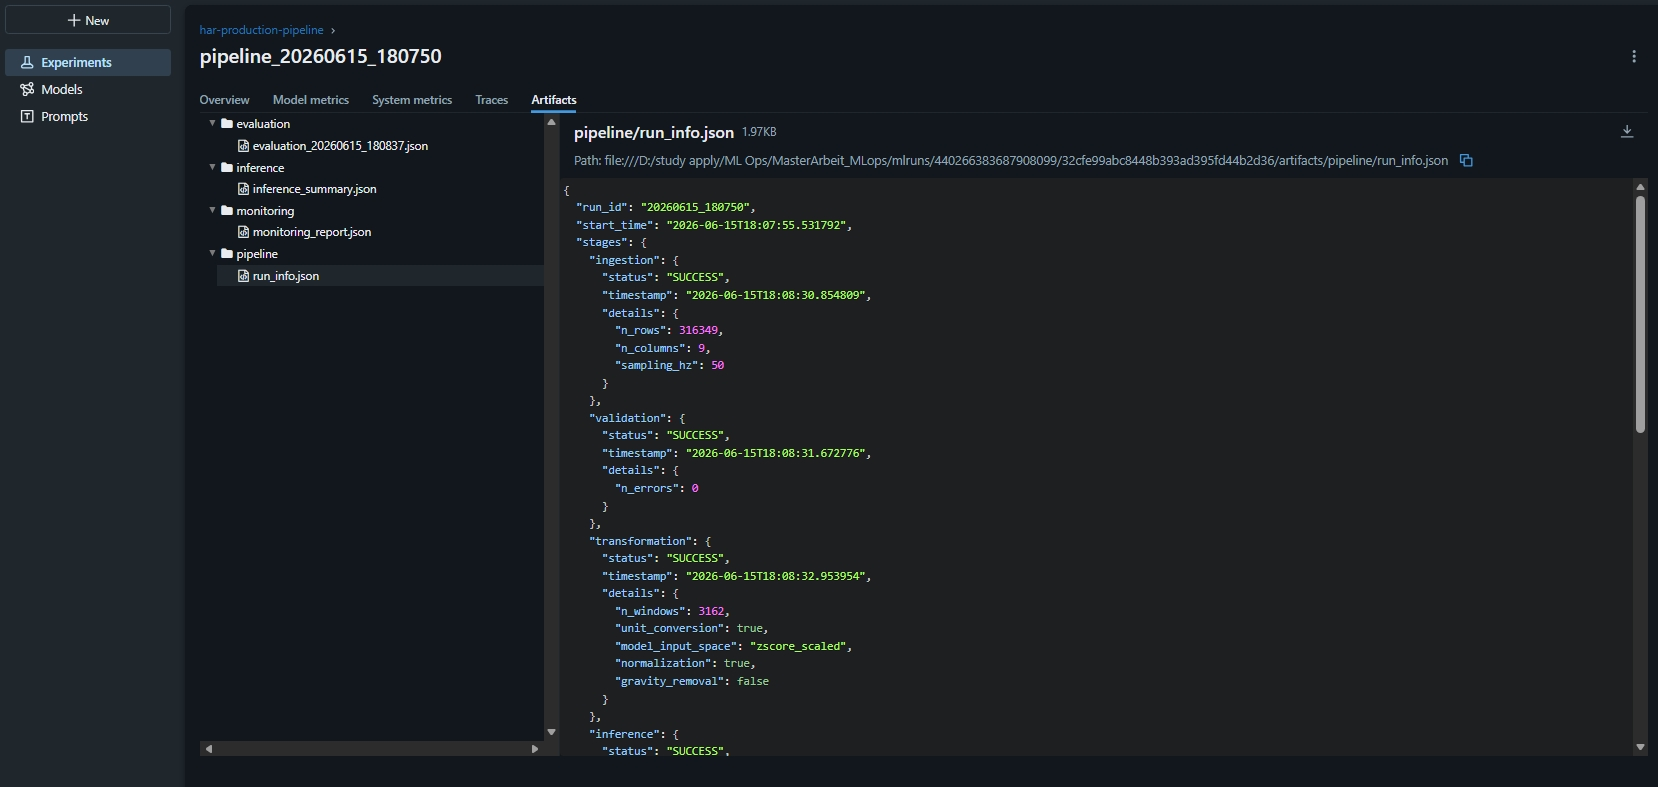
\includegraphics[width=0.94\textwidth]{figures/fig_appF_pipe_artifacts.jpeg}
\caption{\texttt{run\_info.json}: per-stage status and details (rows, windows, unit conversion, model input space), the run-scoped artifact trail.}
\label{fig:appF_pipe_artifacts}
\end{subfigure}
\caption[Har-production-pipeline experiment, part~2]{Har-production-pipeline experiment (continued): the curated stage metrics and the run-scoped artifact trail.}
\label{fig:appF_pipe2}
\end{figure}
\FloatBarrier
